%!TEX root = Report.tex
\chapter{Introduction}\label{sec:introduction}

In this experiment, we measure the flow field of a heated convection cell using "Particle Image Velocimetry" (PIV) technique. PIV is an essential measurement technique in fluid mechanics laboratories in research and industry. It is suitable to a large variety of applications, ranging from microfluids to large fields in wind tunnels.\\

Figure \ref{pic:typsetup} illustrates a typical setup, consisting of a laser source, light sheet optics, the test cell and a camera. Essiantally the displacement of fluid $\Delta x$ is measured over a given time interval $\Delta t$. The position of the fluid is imaged trough the light scattered by solid particles (tracers) illuminated by the laser light sheet.\\

\begin{figure}[H]
\centering
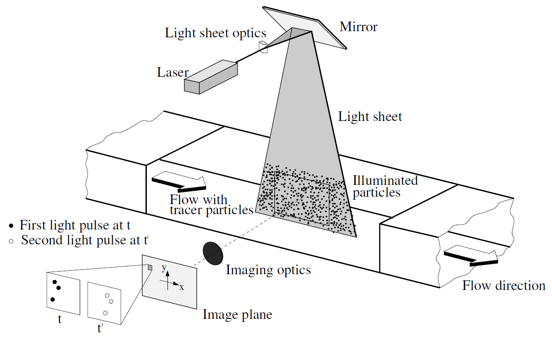
\includegraphics[width=\textwidth]{pics/setup_schematic.png}
\caption{Typical PIV Setup}
\label{pic:typsetup}
\end{figure}

 The light scattered by the particles is recorded on two separate frames. For the evaluation of the acquired data, the images are divided in small areas called "interrogation windows". The displacment vector of the particles between the two images for each interrogation window is then computed using a statistical cross-correlation function. Neighbouring interrogation windows can be partially overlapping in order to reduce spacing between the displacment vectors and to increase resolution. 

